\section{Serialization overheads}


%%TODO \sg{I really like this section for ivy but I don't quite know how to integrate it at the moment.}
% At the end of the day, any consistent memory model requires some form of
% serialization.  Indeed, it is well known that sequential consistency can be
% implemented by ensuring that all operations on a given memory address are
% totally ordered~\cite{ivy}.  In this section, we survey the alternatives
% available in existing RDMA hardware, ranging from optimistic approaches that
% detect and recover from reordering to those that enforce varying degrees of
% serialization.


Passive memory systems suffer from two fundamental sources of overhead: The
additional expense incurred by leveraging any hardware-enforced consistency
semantics at the memory servers, and the costs of resolving conflicts from afar.
Before introducing our approach to avoiding both, we characterize the
potential benefits by quantifying each using microbenchmarks in the context of
Sherman and Clover on our testbed RDMA hardware, NVIDIA Mellanox ConnectX-5
NICs.


%% Sharing remote memory creates a variety of performance problems
%% related to synchronization and serialization. Some problems are
%% system, and algorithm specific, while others are the result of RDMA
%% hardware limitations.  Porting a naive serialization mechanism such as
%% spin locks to remote memory would be prohibitively expensive. Each
%% attempt to require the lock would require a network round trip
%% resulting in a huge latency increase, bandwidth cost and throughput
%% drop. In this section we will avoid using such a straw man comparison
%% and instead highlight the current shortfalls of opportunistic
%% serialization used in Clover as it is state of the art. First we will
%% show why under contention opportunistic concurrency leads to high tail
%% latencies, and low throughput. Then we will discuss how the hardware
%% mechanisms (RDMA CAS) used to achieve serialization are themselves
%% suboptimal.



\subsection{RDMA semantics}

Any client-based contention management scheme requires a certain level
of serialization support at the memory server.  There is a trade-off,
however, between the strength of the guarantees and the costs
associated with implementing them.  RDMA provides two different
classes of guarantees; we summarize both below.

\subsubsection{Atomic requests}

The strongest guarantee available in the RDMA specification is atomicity,
through the use of special atomic requests like fetch-and-add (FAA) and CAS.
Like their traditional CPU counterparts, atomic requests appear to execute at a
single point in time, ensuring a total ordering on all data-dependent
instructions and a partial ordering between all other instructions---i.e., all
other instructions appear to occur strictly before or after the atomic,
regardless of whether they are themselves atomic.

\begin{figure}[t]
  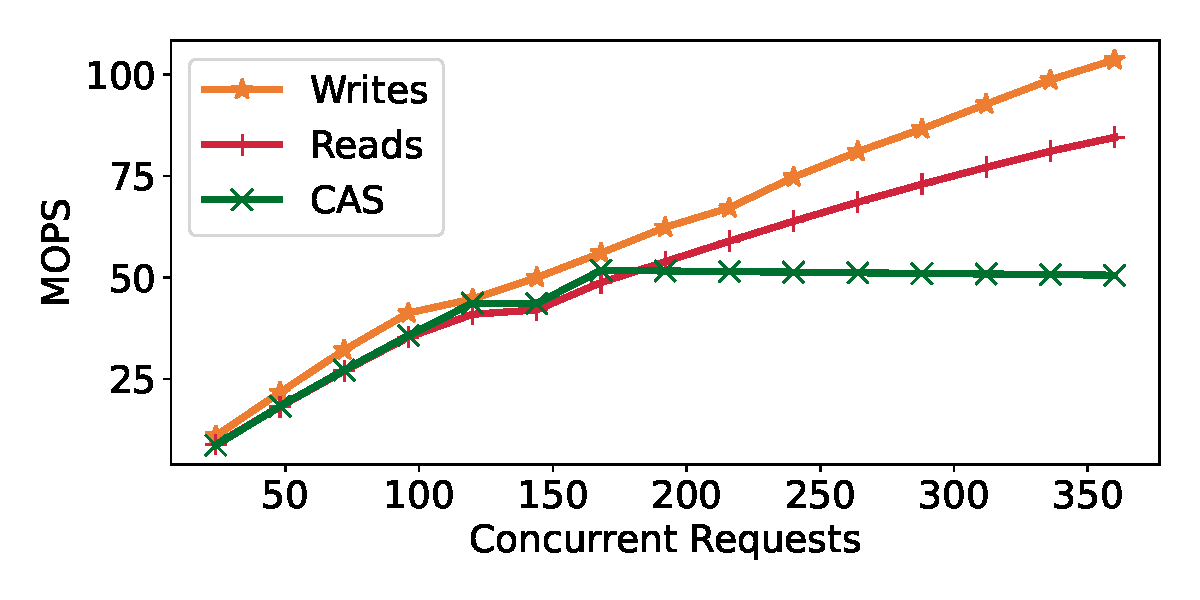
\includegraphics[width=0.485\textwidth]{fig/rdma_concur.pdf}
%  \vskip -0.5em

    \caption{Achieved throughput of RDMA verbs across twenty queue pairs on data
    independent addresses as a function of request concurrency.  When using
    atomic requests, ConnectX-5 NICs can support approximately 2.7 MOPS per
    queue pair, up to about 55 MOPS in aggregate.}

    \label{fig:rdma_concur}
%      \vskip -0.5em
\end{figure}


Atomic primitives enable higher-level serialization structures like locks and
optimistic concurrency schemes. Unfortunately, atomics are famously
expensive~\cite{design-guidelines}, fundamentally because they require mutual
exclusion across all RDMA queue pairs---concurrent read and write operations with a data dependency on the atomic
address must stall until the atomic completes.
%(see Section~\ref{sec:qp_ordering}).
%%
% An RDMA queue pair configured as a reliable connection (RC) acts similarly to a
% TCP connection. Reliable connections provide in order operation serialization
% and ensure at most once semantics. Reliable connections are required by the RDMA
% specification to execute one-sided memory operations like read, write, and CAS.
%
% This work focuses
% exclusivly on RC connections as they do not require and involvement from a CPU
% to execute memory operations.
%
Figure~\ref{fig:rdma_concur} illustrates the scalability of
data-independent (each instruction is issued to an isolated cache
line) atomic operations in comparison to standard reads and writes.
We confirm that the findings of prior
studies~\cite[Fig. 14]{design-guidelines} with older hardware (i.e.,
ConnectX-3) remain true on our ConnectX-5 NICs, namely that atomic
requests scale with non-atomics only to a point.  CAS operations have
a hard performance ceiling, while standard verbs (e.g., read and
write) continue to scale with increased request concurrency.

%In many disaggregated systems operation serialization is performed using RDMA
%atomic operations implemented on a NIC. These
%
% Atomics are expensive both because they can block concurrent RDMA requests and
% because they require multiple round trips over the PCIe bus.
%
%while they execute and require scarce NIC resources.
%
% To provide atomicity, the NIC must ensure that no dependent requests
% are concurrent, dispatch the write, and then wait for the memory operation to
% complete. 


%Whether executed on host or
%NIC-mapped memory, writes on a single queue pair significantly out
%perform atomic operations.

%The time required to complete an atomic is at minimum a PCIe round trip from
%the NIC to main memory, during which time a lock on the NIC guards the memory
%access.

% Lock implementation is both vendor and transport
% specific~\cite{design-guidelines}. In the worst case a barrier is placed on all
% requests resulting in complete head-of-line blocking; in the best case locking
% is per connection and only causes other requests to block when reads or writes
% occur on overlapping ranges virtual memory. Regardless of the implementation,
% atomic requests are likely to be significantly slower than asynchronous
% non-blocking reads and writes.

%% Practically speaking, the performance of atomic operations is limited
%% by the PCIe bus.  In order to provide atomicity, the NIC must ensure
%% that no dependent operations are concurrent, dispatch the write, and
%% then wait for the memory operation to complete.  The separation
%% between the serialization point (NIC) and the data storage (main
%% memory) represents a fundamental overhead to employing atomics.
%% Ideally, the serialization could occur much closer to the memory
%% location itself, as is the case with local CPU instructions and L1
%% cache.

%% RDMA is designed for extremely high throughput and low latency
%% operations. Far memory systems use their verb library to implement
%% remote memory operations. The most common are reads, and writes, with
%% the atomic library being used to implement serialized remote memory
%% accesses. Atomics operations require significantly NIC memory and are
%% substantially slower than default reads and writes.

%% RDMA atomic operations are known to be slow due to their need to make a PCIe
%% round trip. In contrast locks held in SRAM require only a few nanoseconds to
%% perform locking operations. To unlock the full potential of RDMA we convert
%% compare and swap operations to writes in network. While this operation is
%% generally unsafe, by resolving all conflicts, and using RDMA reliable
%% connections, we can ensure all operations succeed and serialization without
%% using RDMA atomic operations.


\subsubsection{Queue-pair ordering}
\label{sec:qp_ordering}

\begin{figure}[t]
    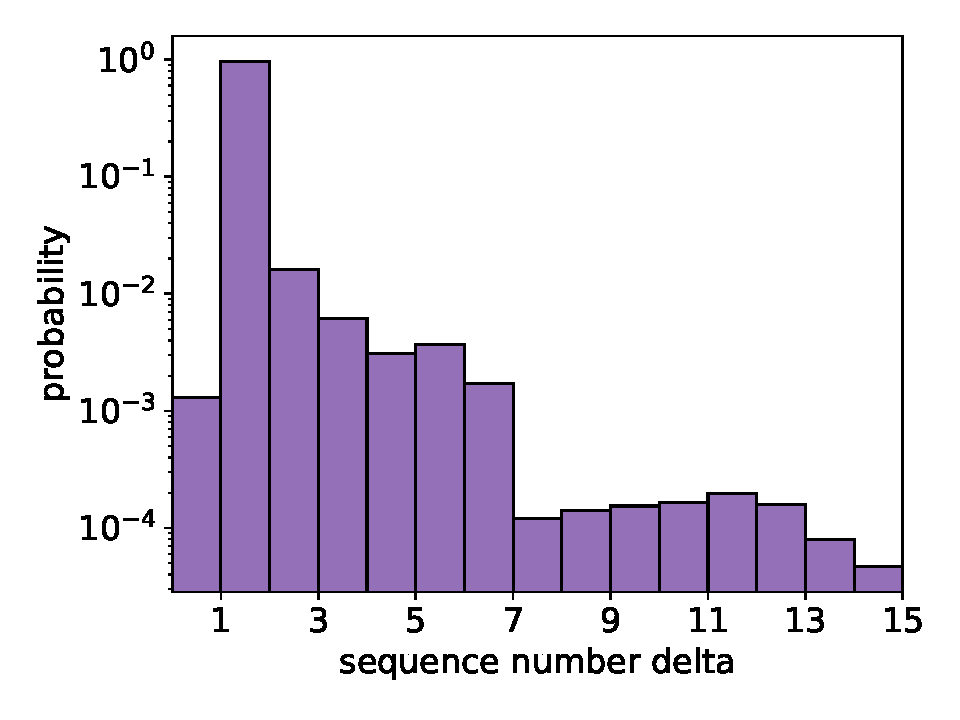
\includegraphics[width=0.485\textwidth]{fig/qp_reordering.pdf}
  \vskip -0.5em    
    \caption{PDF of request reorderings.  Retransmitted requests lead to reordering values of zero.   The majority
    of requests retain their order (delta=1), however reorderings of up to 15
    requests can occur.}
  \vskip -0.5em
    \label{fig:reorder}
\end{figure}

Hence, a scalable far memory system should avoid the use of atomics to the extent possible, instead relying upon lightweight
RDMA verbs.  
%%
Even then, existing hardware does provide some guarantees.  For example,
%RDMA
%provides access to memory hosted on a server that likely utilizes a commodity
all modern hardware memory management units (MMUs) ensure coherent
memory accesses and frequently ensure a total ordering on local memory
requests (i.e., sequential consistency).  Unfortunately, due to the
complexities of today's NUMA architectures and PCIe bus arbitration,
it is possible that memory requests may not be serviced in the order
they are dispatched by the server's NIC.  Similarly, individual RDMA
requests may require multiple memory accesses, potentially leading to
write corruption and read tearing.

Figure~\ref{fig:reorder} shows that this potential reordering is not
just an academic concern, but instead arises with some frequency. In
this example, we issue RDMA read, write and CAS requests at a rate of
one million requests per second to 1,024 different memory locations
according to a Zipf distribution and spread these requests across 32
different queue pairs. Each request is routed through a middlebox that
keeps a global request counter for each RDMA request (i.e., ground
truth regarding request ordering).  We track the order of responses
relative to the order the corresponding request was issued from the
middlebox.  The plot shows the distribution of sequence-number gaps
between responses.  As expected, the vast majority differ by one
(i.e., the same order they were dispatched), but a non-trivial number
are out of order by one to five requests, and some by up to 15.

%% RDMA read and write operations to detect reordering across 1000 keys
%% on a zipf distribution. Specifically we monitor a stream of key value
%% requests in clover and maintain a centralized counter for each
%% packet. When a reply packet is sent from the memory side NIC we
%% compare the sequence of replies with the order that they were issued
%% in. Our experiment monitors requests using a single core, and a single
%% queue on our middle box. Therefore all renderings are the result of
%% reordering on the memory side server, either in the NIC itself or over
%% the PCIe bus.


\begin{figure}[t]
  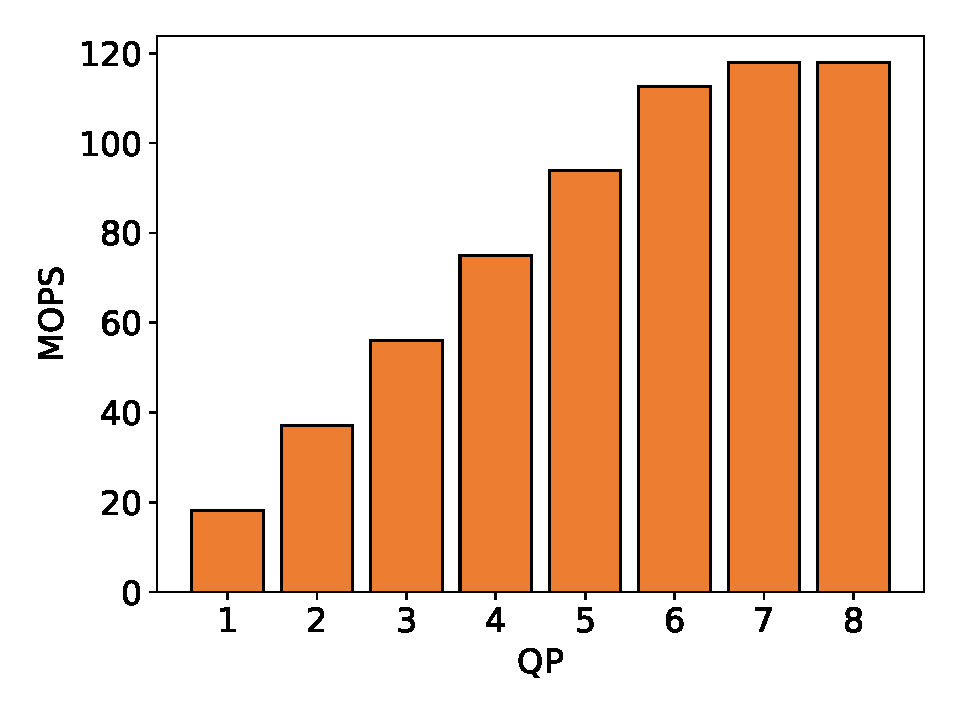
\includegraphics[width=0.485\textwidth]{fig/qp_bottleneck.pdf}
  \vskip -0.5em
\caption{Max throughput as a function of the number of RoCEv2 RC connections. Each QP gets a single
core, and issues in-lined writes. A single connection only offers a fraction of the
total NIC throughput.} 
  \vskip -0.5em
  \label{fig:qp_bottleneck}
\end{figure}

Happily, the RDMA specification provides the ability to provide
partial ordering amongst a subset of requests~\cite{infiniband-spec}.
Specifically, RDMA provides three different types of queue pairs (QP)
with differing ordering---and reliability---guarantees. Unreliable
connections and datagrams (UC \& UD) provide no ordering guarantees
while reliable connections (RC) provide TCP-like in-order processing
of requests on that QP.  As a result, requests on an individual RC are
linearizable with respect to each other, but shared memory accesses
across multiple RC are not.
%
%In order to allow applications to
%reason about and react to this uncertainty,
%
%stipulates that requests made on a
%reliable connection (one-server/one-client queue pair) are guaranteed
%to be executed in the same order as their sequence numbers, similar to
%TCP's transport-layer semantics~\cite{infiniband-spec}.
%~\footnote{while
%IB allows for relaxed ordering here we rely on that feature being
%turned off on the receiver}.
%That is, requests on a given queue pair
%are totally ordered with respect to one another.
% a NIC should ensure that all operations over a given queue pair are
%serviced in the order they arrive.


In general, this can provide sequential consistency if all requests
relating to a given memory location arrive on the same RC queue pair.
Unsurprisingly, however, RC's ordering guarantee comes with its own
scalability limitations.  Figure~\ref{fig:qp_bottleneck} shows that
the performance of individual queue pairs fall far short of line rate
on our NICs; we do not observe full performance until at least seven queue pairs are used simultaneously.  Moreover, as traditionally
conceived, a QP is intended to be established between a single client
and server---limiting its utility in a disaggregated setting.

%% \todo{I think that this was written with a misunderstanding about what the charts were}
%% As expected, when all requests are issued on the same queue pair, they are
%% serviced in order.  Once a non-trivial level of concurrency is reached, however,
%% the reordering becomes significant, with over 7\% of requests to the same
%% address serviced out of order when they are spread across 32 queue
%% pairs.\sg{given a zipf distribution, and 16qp around 3\% of requests are
%% reordered. This is detected by checking the sequence numbers against the known
%% monotonic sequence.}


%\subsubsection{Queue pair bottlenecks}

%%  There are two challenges to restricting requests for a given address
%%  to a single queue pair---one that can be worked around, and one that
%%  must be addressed.  First, queue pairs are established on a
%%  client/server basis, so requests from different clients must arrive
%%  on different queue pairs.  Second, the performance of a single queue
%%  pair on commercial NICs is significantly less than line rate (likely
%%  precisely because of the need to enforce ordering constraints).

\subsection{NIC-based memory}

\begin{figure}[t]
  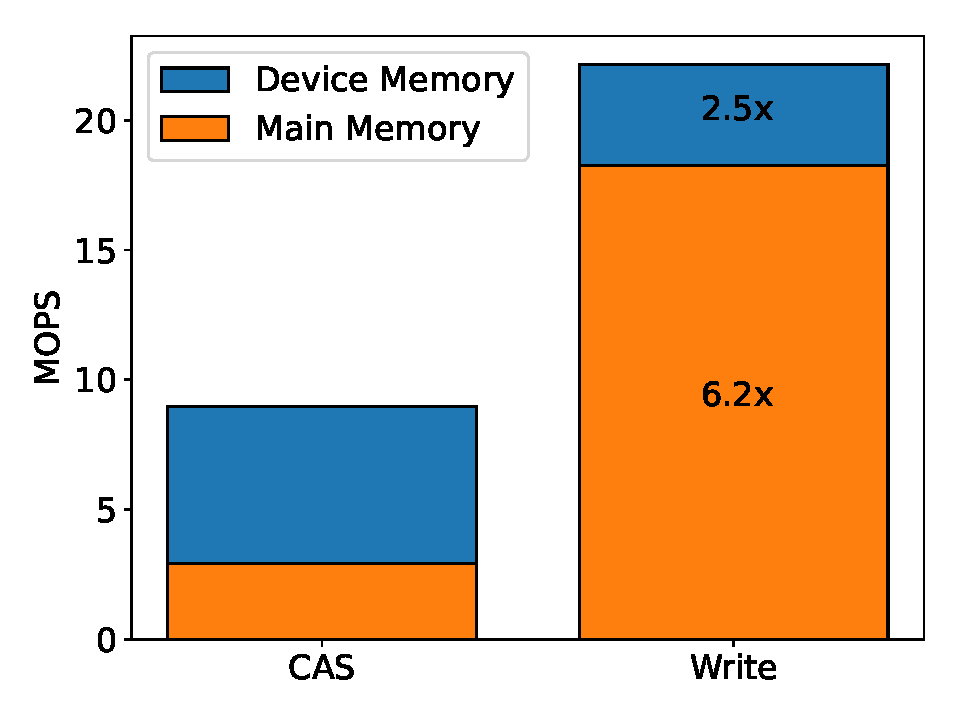
\includegraphics[width=0.485\textwidth]{fig/cas_vs_writes.pdf}
%  \vskip -0.5em

  \caption{ Throughput comparison of serialized RDMA operations in
    NIC-mapped device and main memory. Writes obtain 6.2$\times$ higher
    throughput than CAS in host memory and 2.5$\times$ higher in NIC memory despite being restricted to a single queue pair.  }

    \label{fig:cas_vs_writes}
%      \vskip -0.5em
\end{figure}

Regardless of how operations are serialized,
accesses to main memory on a remote server require multiple PCIe
round trips to
%execute before dependent operations can be unblocked.
complete.
Sherman exploits the fact that newer Mellanox NICs like the ConnectX-5
provide a small region of NIC memory that can be mapped into the
address space of RDMA applications,
%.  Mapping RDMA requests onto NIC memory
removing the remote PCIe overhead for frequently accessed data like its B+Tree locks.
%but still requires atomicity across queue pairs.
Figure~\ref{fig:cas_vs_writes} compares the performance of
serialized CAS and write operations to addresses in main vs.
NIC-hosted device memory. CAS operations are issued across many
queue pairs to achieve maximum throughput while the write operations are
issued on a single queue pair to enforce serialization.
%leverage the serialization provided
%by RDMA's reliable connection abstraction to ensure in-order
%execution.
While the use of NIC-hosted memory boosts CAS throughput
from approximately 3 to around 9 MOPS, write operations remain
dramatically more efficient in either case.


\begin{figure}[t]
    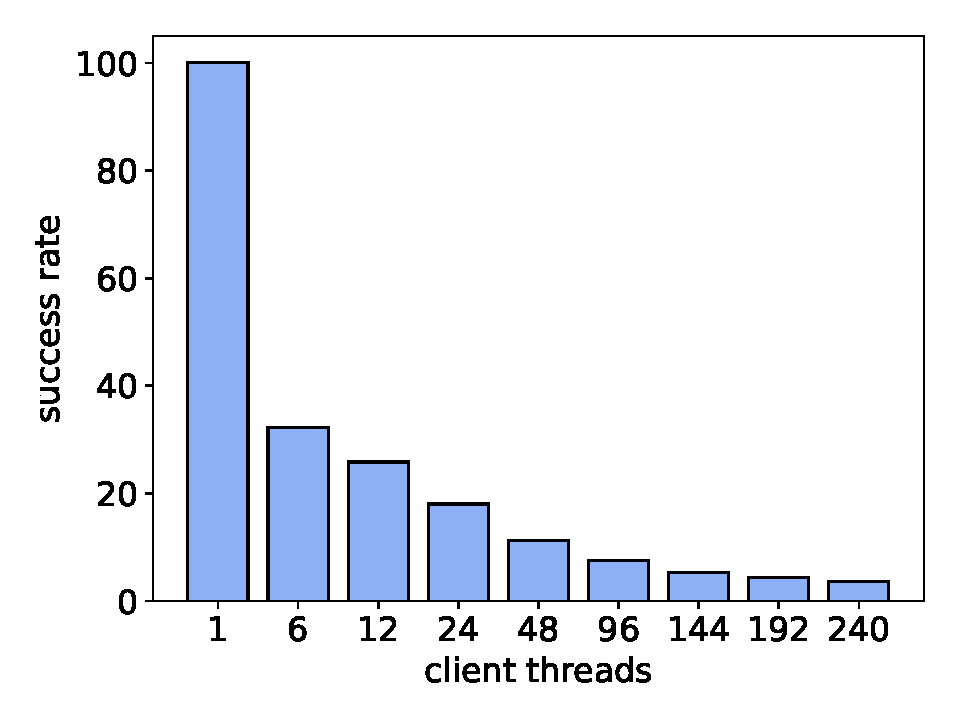
\includegraphics[width=0.485\textwidth]{fig/success_rate.pdf}
    \vskip -0.5em
    \caption{Percentage of successful operations in a
      50:50 read-write workload spread across 1,024 keys according
      to a Zipf(0.99) distribution as more client threads are
      added. At 240 threads less than 4\% of operations succeed.}
      
    \vskip -0.5em
    \label{fig:success_rate}
\end{figure}

\subsection{Optimistic conflict resolution}
%%
Optimistic approaches to concurrency management, while far more
performant than pessimistic ones in the un-contended case, can
frequently be prohibitively expensive when contention is common.  In
general, the conflicting operation(s) must be retried incurring
additional latency and bandwidth.  In some systems, the retry is a
heavyweight, pessimistic operation, leading to a substantial---but
fixed---overhead.  In others, like Clover, subsequent attempts remain
optimistic, resulting in a linear (per-retry) increase in costs.
In the latter case, however, very high rates of contention can lead to
congestion collapse, where a retry is essentially doomed to failure,
dramatically decreasing system throughput.

As a concrete example we consider the costs of contended operations in
Clover.  Recall Clover maintains a linked list for each key and
attempts to read and write to the tail of the list for each
operation. The location of the tail of the list is cached at each
client and used as a hint for subsequent operations.  If the hint is
stale the client obtains an updated tail pointer and retries the
RDMA request.  Figure~\ref{fig:success_rate} shows the percentage of
requests which succeed in a 50:50 read-write workload as a
function of the number of concurrent client threads.

\paragraph{Bandwidth inflation.} 

One of the most direct impacts of failed requests is the bandwidth
overhead of the retries.  Because a Clover operation actually
consists of multiple RDMA requests, the total bandwidth is not
strictly proportional to the failure rate, but rather slightly
sub-linear.  Nevertheless, the expected cost of each operation rises
steadily with contention, which is a function of both the workload and
level of concurrency.  Our measurements show that under contention the
average bandwidth cost of Clover read and write operations can inflate
by 16$\times$ (Figure~\ref{fig:bandwidth_reduction}) when compared
to an optimal scenario in which all operations succeed on their first
try.

\paragraph{Tail latency.}

Perhaps even more significant than the overheads associated with the expected
number of retries is the cost at the tail---namely the latency associated with
those particularly ``unlucky'' requests that fail repeatedly.  Note that these
operations are precisely those for hot memory locations, so likely to be
ones that matter.  Under contention
%(e.g., 50\% write operations with 396 threads)
Clover's 99th-percentile tail latency increases by
over 300$\times$ (Figure~\ref{fig:tail_latency}) in our experiments.

%% Reducing the cost of each operation to exactly 1 attempt can reduce
%% this additional latency by nearly two orders of magnitude.

%% Retried operations result in large throughput drops (2x) and massive
%% increases in tail latency (36x) We correct for these opportunistic
%% failures by caching the location of the most recent writes, and using
%% them to steer operations from old locations to the most up to
%% date. Ensuring that operations do not fail drastically improves
%% overall performance under contention. However some performance is
%% still left untapped as the underlying RDMA hardware has further
%% limitations.
